% !TEX encoding = UTF-8 Unicode
% -*- coding: UTF-8; -*-
% vim: set fenc=utf-8
\documentclass[a4paper,12pt,french]{article}

\usepackage{centrale}

\hypersetup{
  pdftitle={Compte-Rendu TP1},
  pdfauthor={Aymeric ZIMINSKI / Zaryus},
  pdfsubject={Compte-rendu TP},
  pdfproducer={Conversion PDF},
  pdfkeywords={Quelques mots-clés} %
}

\DeclareGraphicsRule{.ai}{pdf}{.ai}{} % Pour insérer des documents .ai
\graphicspath{{./img/} {./eps/} {./fig/}} % Pour ne pas avoir à ajouter eps/ton-image.jpg

% ------------- Packages spéciaux, nécessaires pour ce rapport, à insérer ici ------------- 
\usepackage{minted}


\begin{document}

% --------------------------------------------------------------
%                       Page de garde
% --------------------------------------------------------------

\begin{titlepage}
  \begin{center}

    
\includegraphics[width=0.5\textwidth]{LogoECN.jpg}\\[1cm]

    {\large Réseau}\\[0.5cm]
    {\large Systèmes Embarqués Communiquants}\\[0.5cm]

    % Titre
    \rule{\linewidth}{0.5mm} \\[0.4cm]
    { \huge \bfseries TP : Chat sur socket Unix\\[0.4cm] }
    \rule{\linewidth}{0.5mm} \\[1.5cm]

    % Auteur(es) et encadrant(es)
    \noindent
    \begin{minipage}{0.4\textwidth}
      \begin{flushleft} \large
        \emph{Auteur :}\\
        M. Guillaume \textsc{PIRAUBE}\\
        M. Aymeric \textsc{ZIMINSKI}
      \end{flushleft}
    \end{minipage}%
    \begin{minipage}{0.4\textwidth}
%      \begin{flushright} \large
%        \emph{Encadrants :} \\
%        M.~Prénom \textsc{Nom}\\
%        M.~Prénom \textsc{Nom}
%      \end{flushright}
    \end{minipage}

    \vfill

    % Date en fin de page
    {\large Version du\\ \today}

  \end{center}
\end{titlepage}

% --------------------------------------------------------------
%                    Table des matières
% --------------------------------------------------------------

\thispagestyle{empty}
\tableofcontents
\pagebreak

% --------------------------------------------------------------
%                         Début du corps
% --------------------------------------------------------------

\section{Introduction}

L'objectif de ce TP est de réaliser un chat box sur socket Unix en utilisant le protocole TCP dans un premier temps pour recevoir et envoyer des messages visibles sur le serveur.

Dans un second temps nous allons utiliser le protocole UDP afin de pouvoir envoyer des messages privés. Le tout en utilisant des thread afin de pouvoir gérer la réception de message publique et privé et l'envois de message.


% --------------------------------------------------------------
%                         Partie TCP
% --------------------------------------------------------------

\pagebreak
\section{Partie TCP}
\subsection{Étape 2 — Connexion au serveur}

L'objectif de cette étape est d'établir une connexion TCP avec le serveur central du chat, situé à l'adresse \texttt{169.254.61.46} et qui écoute sur le port \texttt{4242}. La connexion doit être établie \emph{avant} la boucle principale, afin que les threads puissent ensuite utiliser le descripteur de socket pour envoyer et recevoir les messages.

\subsection*{Création de la socket TCP}

\begin{minted}{c}
int sd = socket(AF_INET, SOCK_STREAM, IPPROTO_TCP);
if(sd < 0){
    perror("socket");
    return 1;
}
printf("[CONSOLE] Socket TCP cree\n");
\end{minted}

L'appel système \texttt{socket()} crée un point de communication et renvoie un descripteur de fichier (entier) qui sera utilisé par tous les appels réseau suivants. Les trois arguments sont :
\begin{itemize}
    \item \texttt{AF\_INET} : domaine de communication \textbf{IPv4}.
    \item \texttt{SOCK\_STREAM} : type de socket.
    \item \texttt{IPPROTO\_TCP} : on impose le protocole \textbf{TCP}.
\end{itemize}

\subsection*{Construction de l'adresse du serveur}

\begin{minted}{c}
struct sockaddr_in addr;
addr.sin_family = AF_INET;
addr.sin_port = htons(4242);
addr.sin_addr.s_addr = inet_addr("169.254.61.46");
\end{minted}

\subsection*{Établissement de la connexion}

\begin{minted}{c}
int connect_err = connect(sd, (struct sockaddr*)&addr, sizeof(addr));
if(connect_err < 0){
    perror("connect");
    return 1;
}
printf("[CONSOLE] Socket connecte!\n");
\end{minted}

L'appel \texttt{connect()} déclenche le \textbf{three-way handshake} TCP : le client envoie un segment \texttt{SYN}, le serveur répond par \texttt{SYN-ACK}, puis le client confirme avec \texttt{ACK}. À l'issue de ces trois paquets, la connexion est établie et le serveur envoie immédiatement son message de bienvenue.

C'est exactement l'échange que on a pu observer sur Wireshark (figure \ref{fig:etape2}).

\begin{figure}[H]
    \centering
    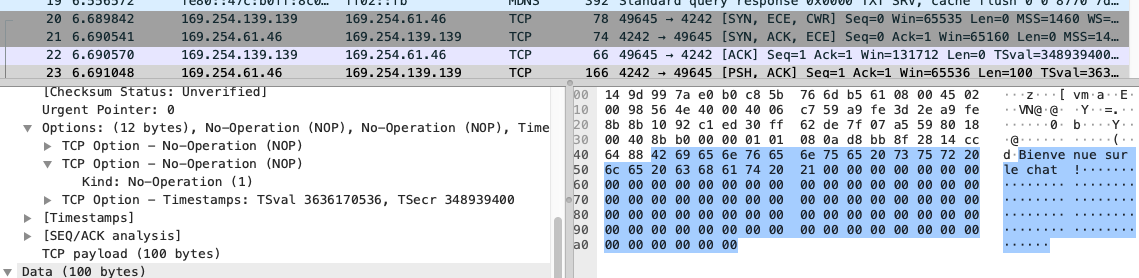
\includegraphics[width=1\textwidth]{etape2.png}
    \caption{Connexion avec le serveur TCP suivi du message de bienvenue.}
    \label{fig:etape2}
\end{figure}


\pagebreak
\subsection{Étape 3 — Réception de messages du chat général}

Le serveur fonctionne en mode \emph{broadcast} : dès qu'un client lui transmet un message, il le rediffuse à tous les clients connectés. Notre tâche consiste à lire en continu ce flux entrant dans la boucle principale. Comme suggéré par l'indice du sujet, c'est le \textbf{thread enfant} (celui pour lequel \texttt{pid[0] == 0} et \texttt{pid[1] == 0}) qui se charge de cette lecture, pour ne pas bloquer la saisie clavier gérée par le parent.

\begin{minted}{c}
if(pid[0] == 0 && pid[1] == 0) {  // thread enfant
    ssize_t lrecv = recv(sd, &buffer, MSG_LEN, 0);
    if(lrecv == 0){
        printf("Client deconnecte\n");
    } else if(lrecv < 0){
        perror("recv");
    } else {
        buffer[lrecv] = '\0';
        printf("%s \n", buffer);
    }
}
\end{minted}

L'appel \texttt{recv(sd, buffer, MSG\_LEN, 0)} lit les données disponibles sur la socket TCP \texttt{sd}. C'est un appel \textbf{bloquant} par défaut : tant qu'aucun octet n'arrive, le thread reste en attente.

\pagebreak
\subsection{Étape 4 — Envoi de messages sur le chat général}

Il faut pouvoir saisir un message au clavier et l'envoyer au serveur. Cette tâche est confiée au \textbf{thread parent} (\texttt{pid[0] != 0} et \texttt{pid[1] != 0}), de sorte à ce que la lecture clavier bloquante n'empêche pas de recevoir les messages.

\begin{minted}{c}
if(pid[1] != 0 && pid[0] != 0){  // thread parent
    /* Lit le contenu */
    scanf(IN_FILT, buffer);


    else {
        /* Pas une commande */
        ssize_t send_err = send(sd, &buffer, sizeof(buffer), 0);
        if(send_err < 0){
            perror("send");
            return 1;
        }
    }
}
\end{minted}

La commande \texttt{send(sd, buffer, sizeof(buffer), 0)} transmet le buffer sur la socket TCP. Le quatrième paramètre (\texttt{flags}) vaut \texttt{0} pour avoir le comportement par défaut.

\begin{figure}[H]
    \centering
    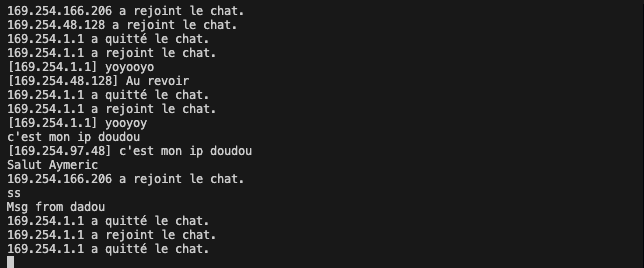
\includegraphics[width=1\textwidth]{etape4.png}
    \caption{Envois et reception du message sur le chat général}
    \label{fig:etape4}
\end{figure}

\pagebreak
\subsection{Étape 5 — Déconnexion du serveur}

L'utilisateur signale son souhait de quitter en tapant la commande \texttt{/q}. Le client doit alors fermer proprement la connexion TCP et libérer toutes les ressources réseau avant de se terminer.

\begin{minted}{c}
if(strcmp(buffer, CMD_QUIT) == 0) {
    /* Commande pour quitter */
    quit = 1;
    printf("Au revoir !\n");
    int shutdown_err = shutdown(sd, SHUT_RDWR);
    close(sd);
    close(sd_UDP_in);
}
\end{minted}

La séquence employée combine \texttt{shutdown()} et \texttt{close()}. Cette distinction est
importante :
\begin{itemize}
    \item \texttt{shutdown(sd, SHUT\_RDWR)} envoie un segment TCP \texttt{FIN} au serveur
    et interdit toute lecture/écriture future sur la socket.
    Cela permet au serveur d'être prévenu \textbf{immédiatement} de la fermeture.
    \item \texttt{close(sd)} libère ensuite le descripteur côté noyau.
\end{itemize}

La variable \texttt{quit} est locale à chaque thread (\texttt{fork()} duplique l'espace mémoire). Mettre \texttt{quit = 1} dans le parent n'arrête \emph{pas} les enfants.

\begin{minted}{c}
if(pid != 0) { // thread parent
    /* Termine le thread enfant */
    kill(pid, SIGTERM);
}
return 0;
\end{minted}

% --------------------------------------------------------------
%                         Partie UDP
% --------------------------------------------------------------
\pagebreak
\subsection{Étape 6 — Création d'une socket d'écoute UDP}

Nous souhaitons maintenant pouvoir envoyer et recevoir des messages privés. Pour se faire, nous commençons par réaliser le socket d'écoute UDP sur le port \texttt{5555}.

\begin{minted}{c}
int sd_UDP_in = socket(AF_INET, SOCK_DGRAM, IPPROTO_UDP);
if(sd_UDP_in < 0){
    perror("socket");
    return 1;
}
printf("[CONSOLE] Socket UDP cree\n");

struct sockaddr_in addr_UDP;
addr_UDP.sin_family = AF_INET;
addr_UDP.sin_port = htons(5555);
addr_UDP.sin_addr.s_addr = INADDR_ANY;

int err_bind_UDP = bind(sd_UDP_in, (struct sockaddr*)&addr_UDP, sizeof(addr_UDP));
if(err_bind_UDP < 0){
    perror("bind");
    return 1;
}
printf("[CONSOLE] Bind UDP passe\n");
\end{minted}

Plusieurs différences notables par rapport à l'étape TCP :
\begin{itemize}
    \item \texttt{SOCK\_DGRAM} (au lieu de \texttt{SOCK\_STREAM}) : on demande un mode
    \textbf{datagramme}. Chaque envoi est un message indépendant, sans connexion préalable,
    sans garantie d'ordre ni de livraison.
    \item \texttt{IPPROTO\_UDP} : protocole UDP.
    \item \texttt{INADDR\_ANY} (valeur \texttt{0.0.0.0}) : on attache la socket à
    \textbf{toutes les interfaces réseau} de la machine. Le client acceptera donc des
    datagrammes arrivant aussi bien par l'interface filaire que par le loopback
    (\texttt{127.0.0.1}), ce qui sera utile pour tester localement à l'étape 10.
    \item \texttt{bind()} associe la socket au port \texttt{5555}.
\end{itemize}

\pagebreak
\subsection{Étape 7 — Détection de la commande de message privé}

Nous allons maintenant implémenter le fait de pouvoir envoyer des messages privés via la commande suivante \texttt{/mp [@IP] [MESSAGE]}, par exemple :
\begin{center}
    \texttt{/mp 169.254.25.1 Ceci est un message prive}
\end{center}

Le fichier \texttt{parse\_command.h} fourni possède la fonction \texttt{parse\_mp} qui permet d'extraire l'adresse IP ainsi que le message. On l'appel donc dans la même section que celle de la commande quit :

\begin{minted}{c}
char ip_addr_mp[50];
char msg_MP[MSG_LEN];
int etat_mp;

etat_mp = parse_mp(buffer, ip_addr_mp, msg_MP);

if(etat_mp == -1){
    printf("Erreur : %s", msg_MP);
}
else if(etat_mp == 1){
    /* Traitement de l'envoi UDP -- voir etape 8 */
}
else{
    /* etat_mp == 0 : ce n'est pas un /mp, on envoie en broadcast TCP */
    ssize_t send_err = send(sd, &buffer, sizeof(buffer), 0);
    /* ... */
}
\end{minted}

Le contrat de retour est synthétisé ci-dessous :
\begin{center}
\begin{tabular}{c|l}
\textbf{Valeur} & \textbf{Signification} \\
\hline
\texttt{-1} & Erreur (compilation regex échouée) \\
\texttt{0}  & La saisie n'est pas une commande \texttt{/mp} \\
\texttt{1}  & La commande \texttt{/mp} a été reconnue et les champs extraits \\
\end{tabular}
\end{center}

\pagebreak
\subsection{Étape 8 — Envoi d'un message privé en UDP}

Une fois la commande \texttt{/mp} implémentée, il faut transmettre le message directement à l'IP cible sur son port \texttt{5555}, sans passer par le serveur. Comme indiqué par l'indice, on crée une \textbf{socket UDP temporaire} dédiée à l'envoi (la socket \texttt{sd\_UDP\_in} de l'étape 6 est réservée à l'écoute).

\begin{minted}{c}
else if(etat_mp == 1){
    // On envoie le MP
    int sd_UDP_out = socket(AF_INET, SOCK_DGRAM, IPPROTO_UDP);

    struct sockaddr_in addr_UDP_out;
    addr_UDP_out.sin_family = AF_INET;
    addr_UDP_out.sin_port = htons(5555);
    addr_UDP_out.sin_addr.s_addr = inet_addr(ip_addr_mp);

    int bytes_sent = sendto(sd_UDP_out, msg_MP, strlen(msg_MP), 0,
                            (struct sockaddr*)&addr_UDP_out,
                            sizeof(addr_UDP_out));
    if(bytes_sent < 0){
        perror("sendto");
    }
    close(sd_UDP_out);
    printf("MP envoye : %s", msg_MP);
}
\end{minted}

L'appel système clé ici est \texttt{sendto()}, qui diffère de \texttt{send()} utilisé en TCP :
\begin{itemize}
    \item \texttt{send()} suppose une socket déjà connectée : la destination est implicite.
    \item \texttt{sendto()} prend \textbf{explicitement} l'adresse de destination dans ses
    deux derniers arguments. C'est indispensable en UDP puisqu'aucune connexion préalable
    n'a été établie : chaque datagramme transporte sa propre adresse cible.
\end{itemize}

À noter que l'on envoie \texttt{strlen(msg\_MP)} octets et non \texttt{sizeof(buffer)} : on ne transmet que le contenu réellement utile, sans le padding du buffer (figure \ref{fig:UDP_MP}).

\begin{figure}[H]
    \centering
    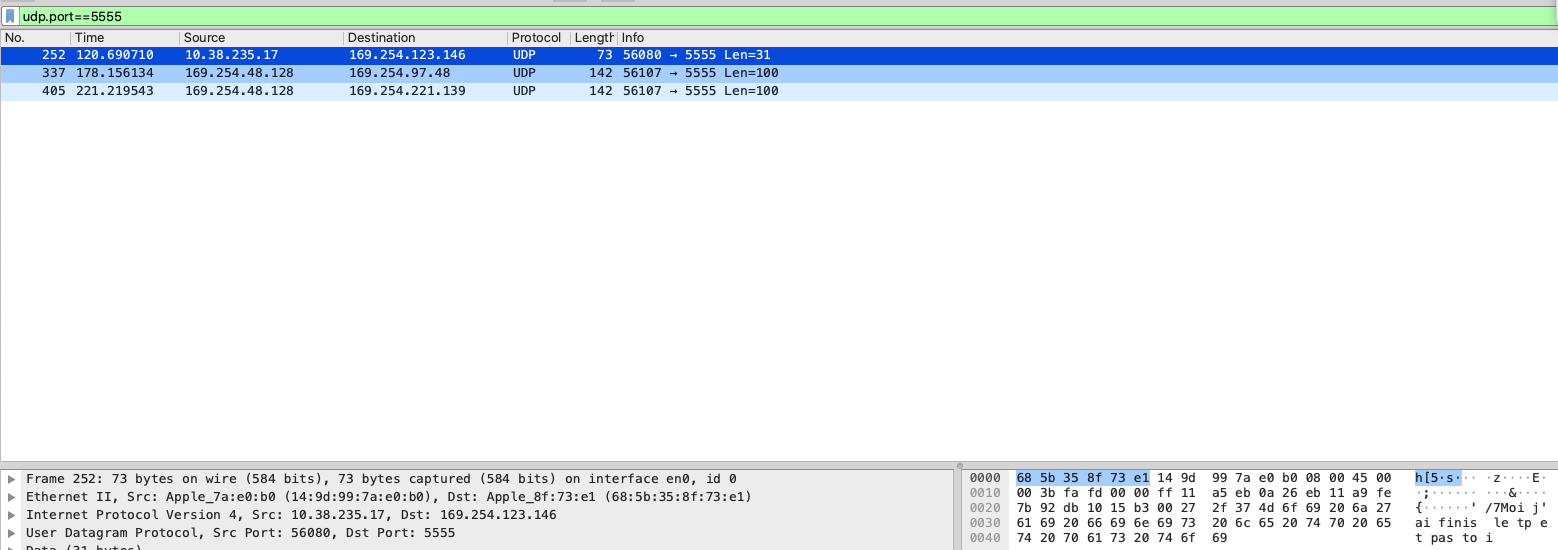
\includegraphics[width=1\textwidth]{UDP_MP.png}
    \caption{Capture Wireshark montrant l'envois d'un message privé}
    \label{fig:UDP_MP}
\end{figure}

\pagebreak
\subsection{Étape 9 — Création d'un thread supplémentaire}

Le client doit maintenant accomplir \textbf{trois} tâches concurrentes : lire le clavier,
recevoir les messages broadcast TCP, et recevoir les messages privés UDP. Avec un seul
thread parent et un seul enfant, on ne pouvait gérer que deux flots bloquants. On ajoute
donc un second \texttt{fork()}, lui aussi exécuté par le parent.

\begin{minted}{c}
int pid[2] = {0, 0};
pid[0] = fork();
if(pid[0] != 0) { // thread parent
    pid[1] = fork();
}
\end{minted}

\subsection*{Analyse des valeurs de \texttt{pid[0]} et \texttt{pid[1]} dans chaque processus}

On peut ainsi synthétiser les processus dans le tableau suivant :

\begin{center}
\begin{tabular}{l|c|c|l}
\textbf{Processus} & \texttt{pid[0]} & \texttt{pid[1]} & \textbf{Rôle dans le client} \\
\hline
Parent              & PID du 1$^{\text{er}}$ enfant & PID du 2$^{\text{nd}}$ enfant & Lecture du prompt + envoi (TCP/UDP) \\
1$^{\text{er}}$ enfant & 0 & 0 & Réception TCP (chat broadcast) \\
2$^{\text{nd}}$ enfant & PID hérité ($\neq$ 0) & 0 & Réception UDP (messages privés) \\
\end{tabular}
\end{center}

Il faut ensuite tuer les deux enfants avant la fin du programme, sinon ils deviendraient orphelins et continueraient à écouter sur les sockets :
\begin{minted}{c}
if(pid[1] != 0) { // thread parent
    kill(pid[1], SIGTERM);
    kill(pid[0], SIGTERM);
}
\end{minted}

\pagebreak
\subsection{Étape 10 — Réception des messages privés}

Le second enfant (identifié par \texttt{pid[1] == 0 \&\& pid[0] != 0}) est dédié à la
scrutation de la socket UDP \texttt{sd\_UDP\_in} attachée au port \texttt{5555} à l'étape 6.

\begin{minted}{c}
if(pid[1] == 0 && pid[0] != 0){
    // Second enfant : reception UDP
    socklen_t addrlen = sizeof(addr_UDP);
    ssize_t recsize = recvfrom(sd_UDP_in, (void*)buffer, sizeof(buffer), 0,
                               (struct sockaddr*)&addr_UDP, &addrlen);
    if(recsize == 0){
        printf("Client deconnecte\n");
    } else if(recsize < 0){
        perror("recv");
    } else {
        buffer[recsize] = '\0';
        printf("%s \n", buffer);
    }
}
\end{minted}

L'appel central est \texttt{recvfrom()}, le pendant UDP de \texttt{recv()}.

\subsection*{Protocole de test local}

Pour valider la chaîne complète sans dépendre d'un autre poste, nous avons suivis les étapes suivantes :
\begin{enumerate}
    \item Faire tourner le premier client \texttt{./client} sur le port \texttt{5555}.
    \item Modifier la valeur du port d'écoute (par exemple \texttt{htons(5556)}), recompiler, et lancer un deuxième client en parallèle.
    \item Depuis le deuxième client, saisir \texttt{/mp 127.0.0.1 Test local} pour s'adresser au deuxième client.
    \item Vérifier que le premier client affiche bien le message reçu.
\end{enumerate}

% --------------------------------------------------------------
%                            Conclusion
% --------------------------------------------------------------

\pagebreak
\section{Conclusion}

Au cours de ce TP, nous avons réalisé un client de chat combinant les protocoles TCP et UDP. Nous avons pu réaliser la première partie sur le protocole TCP, qui permet d'envoyer et de recevoir les messages globaux sur le serveur. Nous avons pu également réaliser la deuxième partie avec le protocole UDP pour la gestion des messages privées sans passer par le serveur en répartissant le tout sur trois processus parallèles pour gérer simultanément la saisie clavier, la réception des messages publics et celle des messages privés.

% --- Biblio par .bib
%\bibliography{ici-ton-fichier-biblio}
%\bibliographystyle{plain-fr.bst}
%\selectlanguage{french}

%\pagebreak
%\appendix
%\begin{appendices}
%\section{}
%\end{appendices}

\end{document}
